\subsection{Если множество $A$ бесконечно, а множество $B$ конечно или счётно, то множество $A \cup B$ равномощно $A$. Равномощность множеств: бесконечных последовательностей из 0 и 1; вещественных чисел; $[0, 1]; [0, 1)$; множества всех подмножеств натуральных чисел. Равномощность отрезка и квадрата.}
\textbf{Если множество $A$ бесконечно, а множество $B$ конечно или счётно, то множество $A \cup B$ равномощно $A$.}\\

Пусть $A$ - бесконечно, $B$ - не более, чем счетное. Тогда $A \cup B \sim A$.\\

\noindent \textbf{Доказательство:} \\

$B' = B \backslash A$, $B'$ - не более, чем счетное. Очевидно, что $A \cup B = A \cup B'$, но $A$ и $B'$ - не пересекаются.
Так как $A$ - бесконечно, то $\exists C \subseteq A, C$ - счетно. Так как $C \cup B'$ - счетно, то $C \sim C \cup B'$. Значит
$\exists f : C \to C \cup B'$ - биекция.

\begin{figure}[H]
\centering
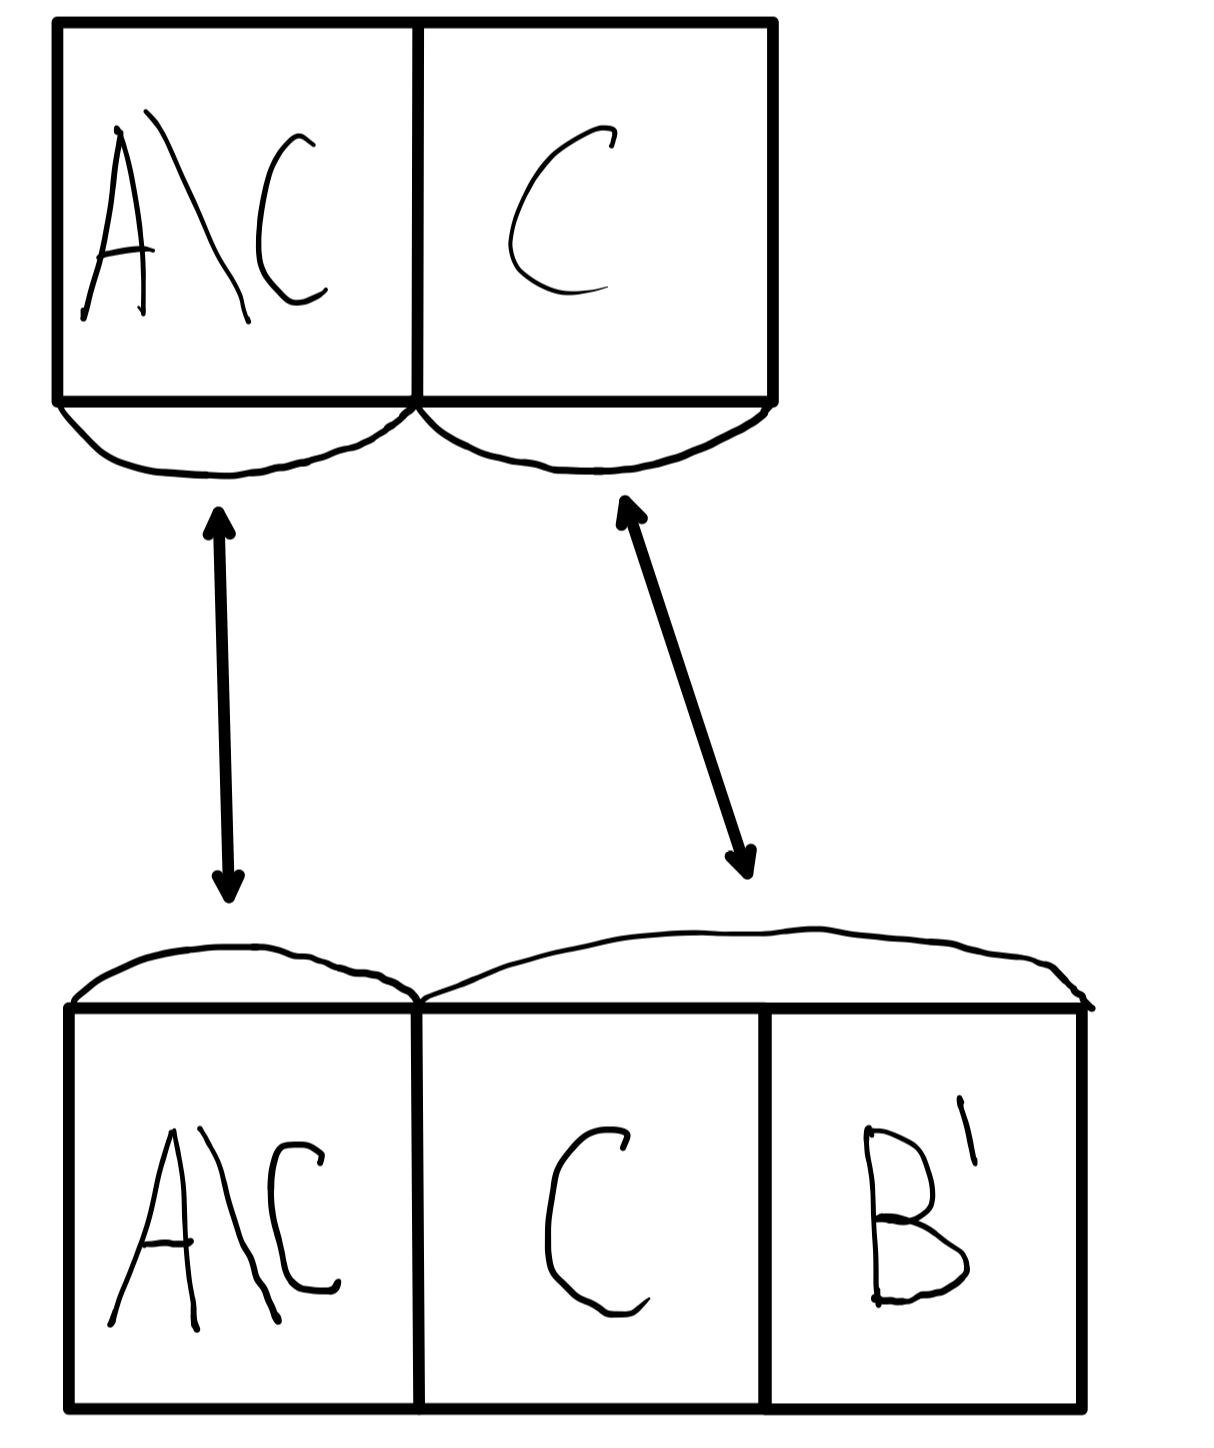
\includegraphics[width=0.3\linewidth]{images/question16.png}
\caption{иллюстрация биекции}
\end{figure}

Теперь просто построим биекцию $g : A \to A \cup B'$.

\begin{equation*}
    g(a) = \begin{cases}
        f(a), \text{если } a \in C\\
        a, \text{иначе}
    \end{cases}
\end{equation*}

\textbf{Равномощность множеств: бесконечных последовательностей из 0 и 1; вещественных чисел; $[0, 1]; [0, 1)$; множества всех подмножеств натуральных чисел.}\\

Нужно доказать: $\mathbb{B}^{\infty} \sim [0, 1) \sim [0,1] \sim \R \sim 2^{\N}$\\



\textbf{Равномощность отрезка и квадрата.}\\